\documentclass[a4paper]{article}
\usepackage{amsmath}
\usepackage{url}
\usepackage{graphicx}
\usepackage[margin=1.2in]{geometry}

\title{\vspace{-3em} Exercise 3\\[10pt] \large FY8503 Advanced theoretical physics\\  Transport modelling with Stochastic differential equations}

\author{September 25, 2023}
\date{}

\begin{document}
\maketitle

{\bf Disclaimer:} I tried googling, asking around, and reading a bit in Kloeden, Platen \& Schurz, to see if I could find an example of a situation where strong convergence is more important than weak convergence. The problems below are made based on this, but when I solved the problems I didn't find any obvious benefit of using higher order of strong convergence. I will keep looking. (And the problems are of course still relevant and useful practice.)

\section*{Problem 1}

Here, we will look at a concept called first exit, or first passage. We will model a large number of solutions to the SDE for geometric Brownian motion,
\begin{align}
    \label{eq:geometric}
    \mathrm{d} X_t = \alpha X_t \, \mathrm{d}t + \beta X_t \, \mathrm{d}W_t,
\end{align}
and find the time it takes for each solution to first reach a value $X_\mathrm{max}$. The time this takes is sometimes called the stopping time, the hitting time, or the time to first passage, and probably other things as well. An example where this comes up is in finance, where the price of an asset is modelled as a stochastic process, and you wish to sell the asset once the price reaches a certain level.


\subsubsection*{Task a}
Use $\alpha=1.5$, $\beta=1$, $X_0=1$, $X_\mathrm{max}=15$, and solve \eqref{eq:geometric} with the Euler-Maruyama method. For each solution, find the first time $t$ where $X_t \geq X_\mathrm{max}$, and plot the distribution of these times. Note that we cannot know ahead of time how long it takes for all the solutions to reach $X_\mathrm{max}$, hence you will somehow have to take this into account in your code.

\subsubsection*{Task b}
Repeat the calculations above, using the Milstein scheme instead. Compare the two distributions. You may have to try different timesteps and numbers of particles until you find something that looks reasonable.

\subsubsection*{Task c}
Euler-Maruyama has order of convergence 0.5 and 1 in the strong and weak sense, while Milstein has order 1 for both. Think about how you can investigate whether or not the higher order of strong convergence of the Milstein scheme makes a difference to the results of the tasks above. Feel free to try different parameter values ($\alpha$, $\beta$, $X_0$, and $X_\mathrm{max}$) if that helps.


\section*{Problem 2}

Here we will look at a version of the Duffing-van der Pol oscillator, and try some calculations as described on pages 222--225 in Kloeden, Platen \& Schurz. The oscillator is described by two coupled SDEs:
\begin{align}
    \label{eq:vdp}
\mathrm{d}X &= V\, \mathrm{d}t \\
\mathrm{d}V &= \big(X(\alpha-X^2) - V^2\big) \mathrm{d}t + \sigma X \, \mathrm{d}W_t,
\end{align}
where $\alpha$ and $\sigma$ are constants.


\subsubsection*{Task a}

Let $\alpha=1.0$ and $\sigma=0.2$. As initial values, use $V_0=0$, and let $X_0$ take 10 different values, equally spaced from $-4$ to $-2$. Solve the SDE from $t=0$ to $t=10$. Show your results by plotting $V$ as a function of $X$. The result should look something like the figure below, where the trajectories are all attracted to either the point $(-1, 0)$ or $(1, 0)$.

\begin{figure}[!!h]
    \centering
    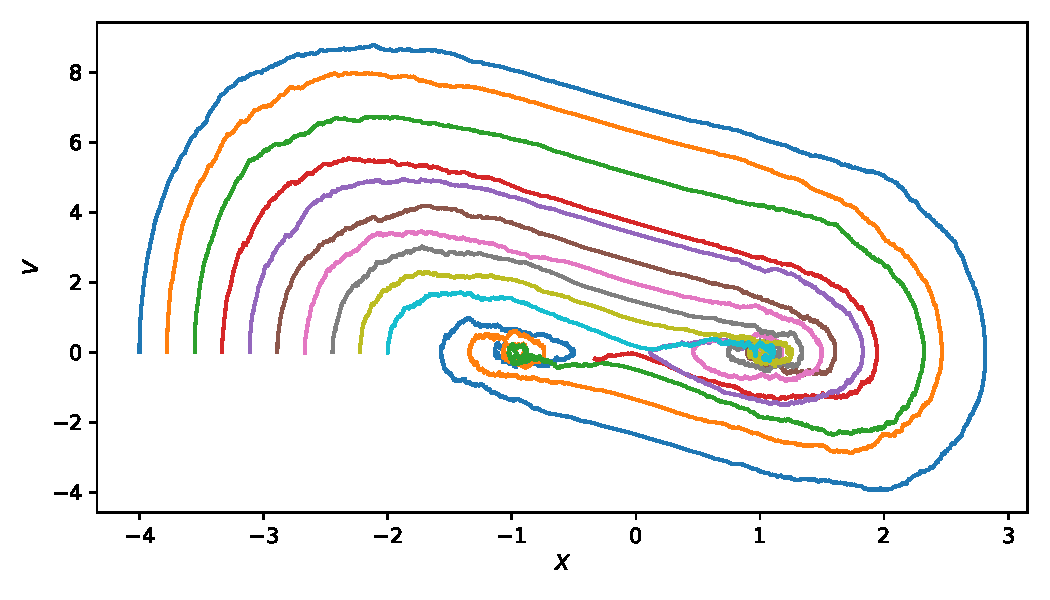
\includegraphics[width=0.9\textwidth]{fig/exercise3_duffing_vdp.pdf}
\end{figure}


\subsubsection*{Task b}

If we solve for several diffent initial conditions, $X_0$, with \emph{the same realisation} of $W_t$, we should be able to observe that the solution $X_t$ varies smoothly with the changing initial condition. This suggests that the trajectories starting from neighbouring initial conditions should not cross (in the $X-V$-plane). According to Kloeden, Platen \& Schurz (bottom of page 222), preserving this property is an indication of the accuracy of ``a strong numerical scheme''\footnote{It is not completely clear if they mean ``strong'' as in a scheme with a high order of strong convergence, of if they use the word ``strong'' more casually, as a synonym for ``good''.} They suggest investigating this by plotting $X_t$ as a function of time, and seeing that the solutions split nicely into two groups, which end up close to either $X=-1$ or $X=1$.

Solve Eq.~\eqref{eq:vdp} for some number (50 or 100, say) of initial conditions, with $X_0$ evenly spaced between $-4$ and $-2$, and $V_0=0$, and solve from $t=0$. Present the solutions by plotting $X_t$ as a function of time. Try different timesteps, and try both Euler-Maruyama and Milstein, and see if there are any differences between the schemes.


\subsection*{References}

Kloeden, Platen \& Schurz, 1997, \emph{Numerical Solution of SDE Through Computer Experiments}, Springer-Verlag, Berlin, Heidelberg, corrected second printing.
\url{https://link.springer.com/book/10.1007/978-3-642-57913-4}





\end{document}
